\section{Suffix Trees}

\begin{Definition}
  A \defi{suffix tree}{Suffix Tree} $\mathcal{T}$ for a string $S$ is the suffix trie of $S$ where each unary path is converted into a single edge. Those edges are labeled with the concatenation of the characters from the replaced edges. The leaves of the suffix tree store the text position where the corresponding suffix starts.
\end{Definition}

\begin{Example}
  Figure~\ref{fig:suffixTreeExample} shows the suffix tree for the string "banana\$". It contains only $11$ vertices compared to the $23$ vertices of the suffix trie.
  \begin{figure}[htb]
    \centering
    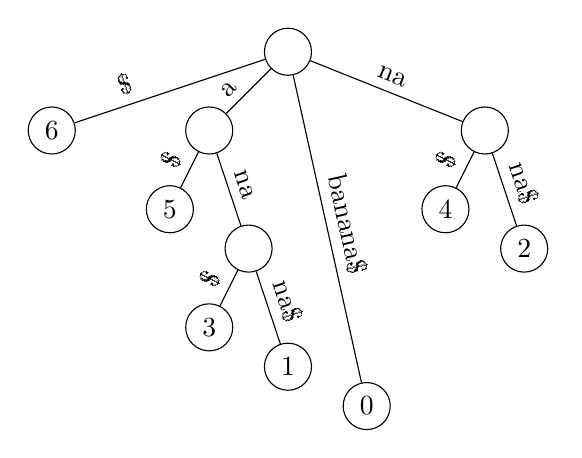
\begin{tikzpicture}
  \tikzstyle{vertex}=[circle,draw,minimum size=17pt,inner sep=0pt]
  \node[vertex] (epsilon) at (0,0) {};

  \node[vertex] (d) at (-3,-1) {6};
  \draw (epsilon) -- (d) node[above,sloped,pos=0.7] {\$};

  \node[vertex] (a) at (-1,-1) {};
  \draw (epsilon) -- (a) node[above,sloped,pos=0.7] {a};

  \node[vertex] (ad) at (-1.5,-2) {5};
  \draw (a) -- (ad) node[above,sloped,pos=0.5] {\$};

  \node[vertex] (ana) at (-0.5,-2.5) {};
  \draw (a) -- (ana) node[above,sloped,pos=0.5] {na};

  \node[vertex] (anad) at (-1,-3.5) {3};
  \draw (ana) -- (anad) node[above,sloped,pos=0.5] {\$};

  \node[vertex] (ananad) at (0,-4) {1};
  \draw (ana) -- (ananad) node[above,sloped,pos=0.5] {na\$};

  \node[vertex] (bananad) at (1,-4.5) {0};
  \draw (epsilon) -- (bananad) node[above,sloped,pos=0.5] {banana\$};

  \node[vertex] (na) at (2.5,-1) {};
  \draw (epsilon) -- (na) node[above,sloped,pos=0.5] {na};

  \node[vertex] (nad) at (2,-2) {4};
  \draw (na) -- (nad) node[above,sloped,pos=0.5] {\$};

  \node[vertex] (nanad) at (3,-2.5) {2};
  \draw (na) -- (nanad) node[above,sloped,pos=0.5] {na\$};
\end{tikzpicture}

    \caption{The suffix tree for the string "banana\$".}
    \label{fig:suffixTreeExample}
  \end{figure}
\end{Example}

The suffix array can be constructed in time $\mathcal{O}(n)$ with algorithms by \textsc{Weiner}\cite{Weiner1973}, \textsc{McCreight}\cite{McCreight1976} or \textsc{Ukkonen}\cite{Ukkonen1995}. It needs $\mathcal{O}(n\log n + n\log \sigma)$ bits. The first summand is the space needed for the pointers to the children and the indices stored in the leaves. The second summand is the space needed for the edge labels. To achieve this space, the edge labels must not be stored explicitly. Instead we can store pointers to the first and last position of the label in the text.

In practice, a suffix tree needs more than $20$ times the space of the original text. Based on the required functionality, this can even be worse.
